\begin{figure}[t]
	\begin{center}
		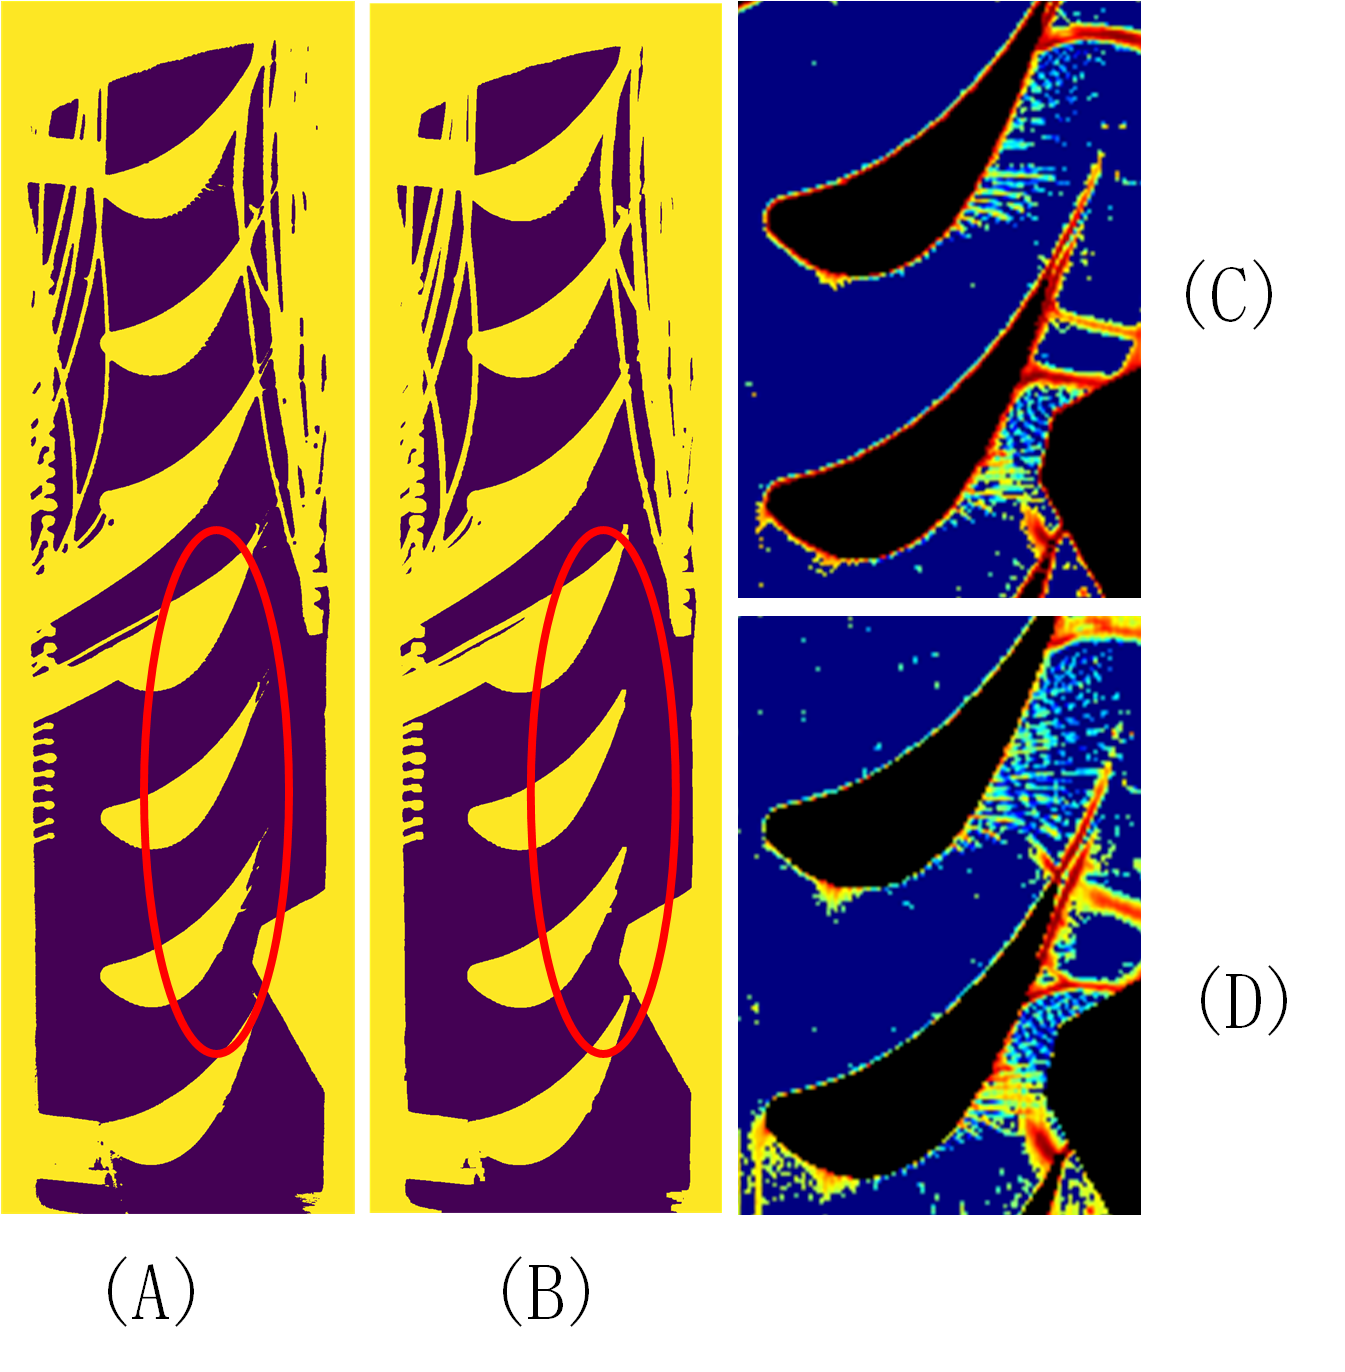
\includegraphics[width=0.75\linewidth]{src/rigid}
	\end{center}
	\caption{(A)(B)分别为$M_r$膨胀腐蚀操作前与操作后,(C)(D)分别为经过处理前与处理后的不同结果. 可以看到膨胀腐蚀操作去除了孤立点(红色圈出), 并且能有效改善叶片边缘处像素分类为Flow区域并带入渲染造成的红圈错误.}
	\label{fig:rigid}	
\end{figure}